\section{Dynamic similarity}


One of the main guiding principles in fluid mechanics is \emph{dynamic
  similarity}. The main question is under what conditions flows around
or in \emph{geometrically similar} geometries of different size are
similar in terms of topology.

Dynamic similarity analysis is not an academic exercise but allows us
to tackle some important questions concerning performance of an
airfoil, a machine, \ldots, in particular
\begin{itemize}
\item what are the number of independent parameters that determine
  performance ?
\item how can we rescale a design ?
\item how can we correct for non-standard atmospheric test conditions
  ?
\item can we a priori choose an optimal configuration as a function of
  operating conditions ?
\end{itemize}

\subsection{Intuitive derivation}

Consider for instance the flow around airfoils. Geometrical similarity
implies that the angle of the flow with respect to the airfoil needs
to be the same. For simplicity, we considered the air flow to be
incompressible, \ie its density $\dens$ is constant. The Navier-Stokes
equations reduce to
\begin{align*}
  \dive \velV = 0 \\
  \ddt{\dens \velV} + \dive \dens \velV \velV + \grad p = \mu
  \left(\grad \velV + \grad \velV^T\right)
\end{align*}
which are solved for both velocity $\velV$ and pressure $p$. We can
now non-dimensionalize the equations using the airfoil chord $C$, the
density $\dens$ and the upstream velocity $\vel_\infty$ as reference
scales. Dividing the first equation by $\vel_\infty / C$, and the
second by $\dens \vel_\infty^2/C$, we arrive at the non-dimensional
form
\begin{equation}
  \begin{split}
  \diveP \velV^\prime = 0 \\
  \ddtP{\velV^\prime} + \diveP \velV^\prime \velV^\prime + \gradP p^\prime = \frac{1}{Re} 
  \left(\gradP \velV^\prime + \gradP \velV^{\prime T}\right)
  \end{split}
  \label{eq:nonDimNavierStokes}
\end{equation}
where $Re_C$ is the \emph{Reynolds number}
\begin{align*}
  Re_c = \frac{\rho \vel_\infty C}{\mu}
\end{align*}
and $\velV^\prime$ and $p^\prime$ are the non-dimensional velocity and
pressure. The flow around the airfoil remains dynamically similar as
long as the non-dimensional Reynolds number, and therefore the form of
the equations \ref{eq:nonDimNavierStokes}, is the same. This is
illustrated in figure \ref{fig:naca4412_flow}
\begin{figure}[!h]
  \centering
  \begin{subfigure}{0.49\textwidth}
    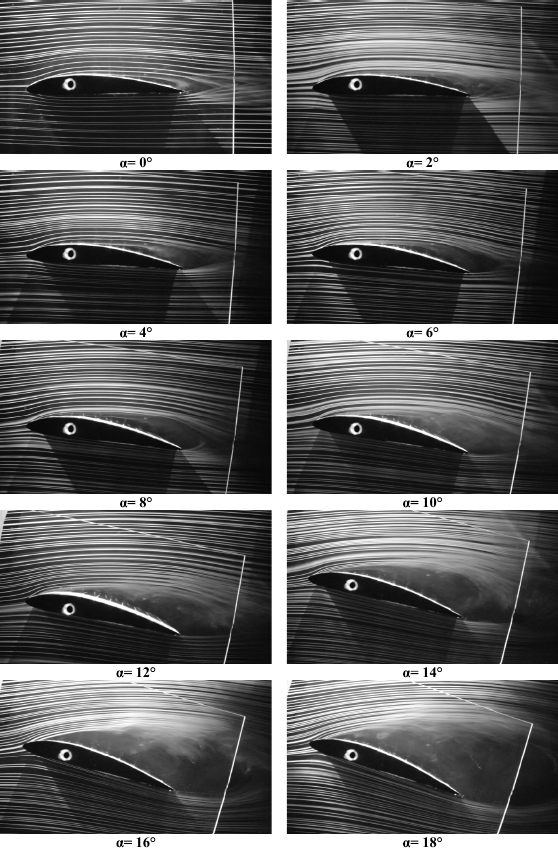
\includegraphics[height=0.52\textheight]{naca4412Koca_Re25000.png}
    \caption{$Re_c = 25000$}
  \end{subfigure}
  \begin{subfigure}{0.49\textwidth}
    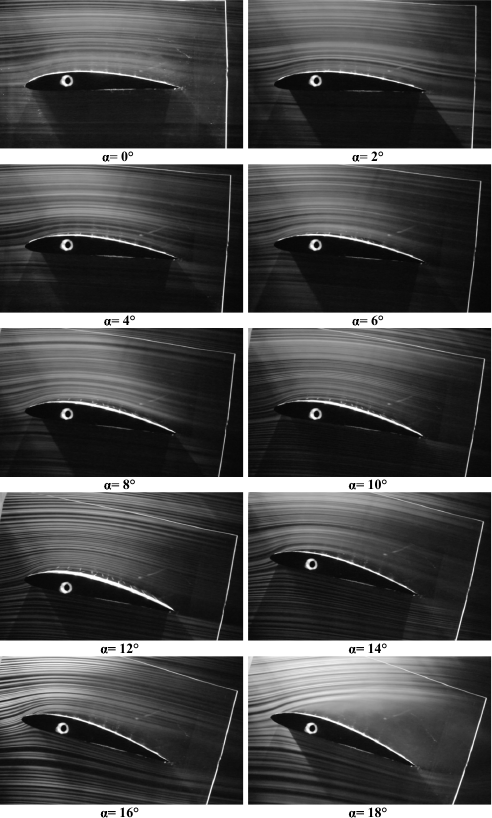
\includegraphics[height=0.52\textheight]{naca4412Koca_Re75000.png}
    \caption{$Re_c = 75000$}
  \end{subfigure}
  \caption{Dependence of the flow around the NACA4412 airfoil from the
    chord Reynolds number $Re_c$. From Koca \etal \cite{KGA+18}}
  \label{fig:naca4412_flow}
\end{figure}
%
\begin{figure}[!h]
  \centering
  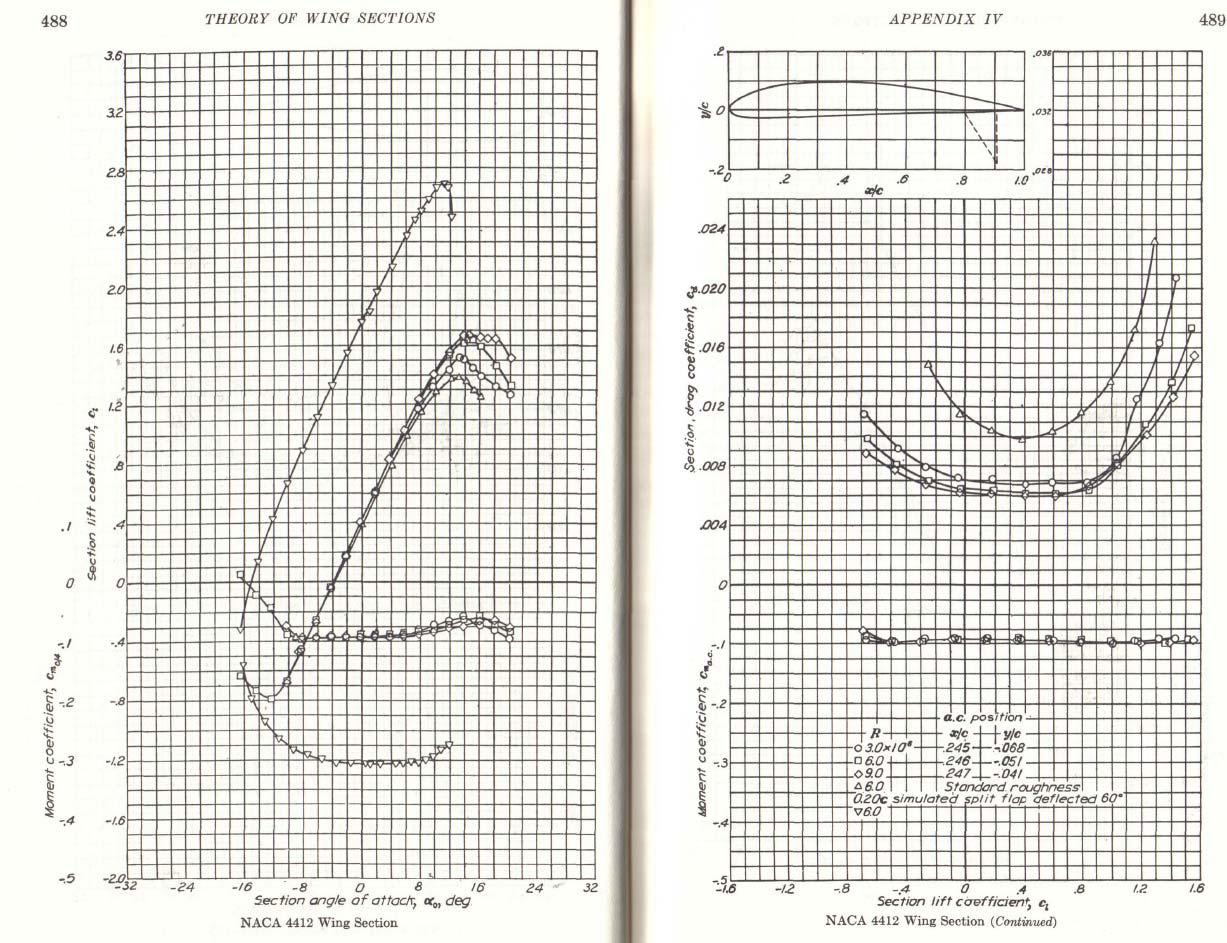
\includegraphics[width=\textwidth]{principles/naca4412_1.png}
  \caption{NACA4412 airfoil lift $C_L$, drag $C_D$ and moment
    coefficient $C_M$. From Abbott and von Doenhoff
    \cite{AbbottDoenhoff}}
  \label{fig:naca4412}
\end{figure}
%
We can easily see that the dimensional pressure and viscous stress
scale as the $\dens\vel_\infty^2 $. Therefore the lift $\forceV_L$ and
drag $\forceV_D$ scale as $\dens\vel_\infty^2~SC$. Choosing the
dynamic pressure as reference, we define
\begin{align*}
  \force_L &= C_L(Re_C,\alpha) \cdot \frac{1}{2} \dens \vel_\infty^2 \cdot C S \\
  \force_D &= C_D(Re_C,\alpha) \cdot \frac{1}{2} \dens \vel_\infty^2 \cdot C S
\end{align*}
with define the lift $C_L$ and drag coefficient $C_D$. Similarity can
therefore be used to tabulate airfoil performance, under the form of
force coefficients, irrespective of upstream velocity, fluid density
or viscosity and airfoil dimensions.

\subsection{The Buckingham $\pi$ theorem}

We can determine how many independent non-dimensional parameters are
relevant using the Buckingham $\pi$ theorem. Assume the a physical
process which is described by a relation between n parameters $Q_i$
\begin{align*}
  f(Q_1,\ldots,Q_n)=0
\end{align*}
Suppose $Q_i$ can be expressed as a function of k independent
fundamental physical dimensions $D_j$, then the process can be reduced
to a relation between $N=n-k$ dimensionless parameters $\Pi_j$:
\begin{align*}
  g(\Pi_1,\ldots,\Pi_N) = 0
\end{align*}

The theorem can be understood easily in the following way. Any of the
$n$ physical variables $Q_i$ can be expressed in terms of $k$ physical
dimensions $D_j$
\begin{align*}
  Q_i \sim \prod_{j=1}^k D_j^{A_{ij}}
\end{align*}
Consider any other combination $V$ of the physical variables
\begin{align*}
  V &\sim \prod_{i=1}^n Q_i^{d_i} = \prod_{j=1}^k D_j^{v_j} 
\end{align*}
This relation can be written down in matrix form as
\begin{align*}
  \begin{bmatrix} v_1 \ldots v_k \end{bmatrix} = 
  \begin{bmatrix} d_1 \ldots d_n \end{bmatrix} \cdot 
  \begin{bmatrix} A_{11} & \ldots & A_{1k} \\ \ldots \\ A_{n1} & \ldots & A_{nk} \end{bmatrix}
\end{align*}
The quantity $V$ is not dependent on dimension $D_i$ if $v_i=0$; it is
non-dimensional if $v_i=0~,~\forall i$. This means that
$\begin{bmatrix} d_1 \ldots d_n \end{bmatrix}$ is in the null-space of
$A$. As the rank of $A$ is equal to the number of independent
dimensions $k$, its null-space has the dimension $n-k$, meaning that
only so many independent non-dimensional combinations can be found.

\subsection{Application to the airfoil}

In the case of the airfoil, the forces are determined by free stream
velocity $\vel_\infty$, the flow angle $\alpha$, airfoil chord $C$,
air density $\dens$ and viscosity $\dynVisc$, giving a relationships
between 6 physical variables:
\begin{align*}
  \force_L &= \force_L(\vel_\infty,\alpha,C,\dens,\dynVisc) \\
  \force_D &= \force_D(\vel_\infty,\alpha,C,\dens,\dynVisc)
\end{align*}
All of the quantities can all be expressed in terms of 3 dimensions,
namely length, time and mass. Therefore, the force relations can be
reduced to expressions involving 3=6-3 non-dimensional parameters:
\begin{align*}
  C_L &= C_L(Re,\alpha) \\
  C_D &= C_D(Re,\alpha) 
\end{align*}
We furthermore see that by using non-dimensional performance
parameters, we remove the dependence on the testing conditions, in
particular the atmosphere (\ie air density and viscosity).

\subsection{Use of similarity}

\begin{figure}[!h]
  \centering
  \begin{subfigure}{0.24\textwidth}
    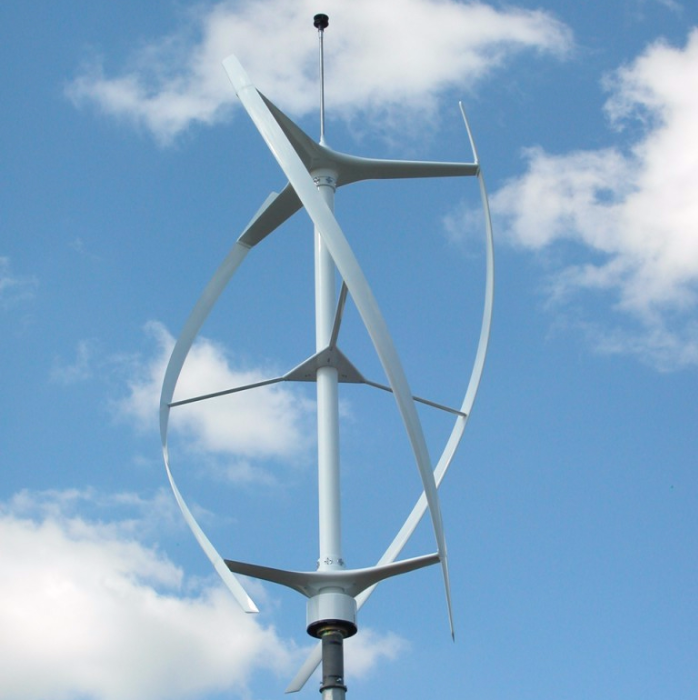
\includegraphics[width=\textwidth]{principles/vawt.png}
    \caption{Geometry}
    \label{fig:vawtGeometry}
  \end{subfigure}
  \begin{subfigure}{0.37\textwidth}
    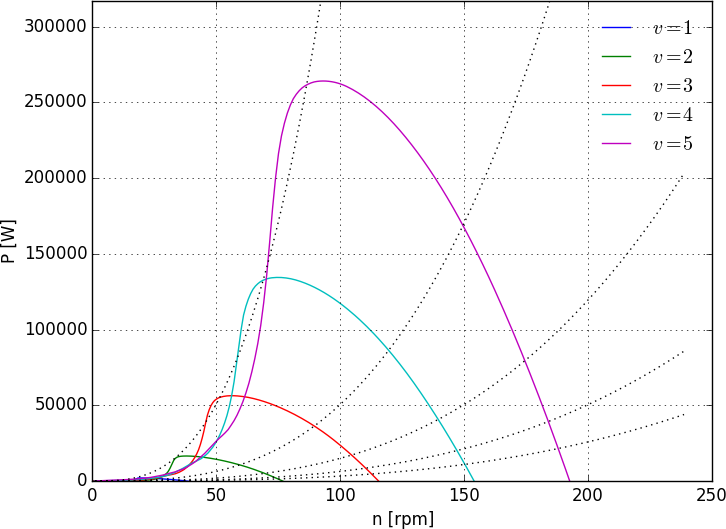
\includegraphics[width=\textwidth]{principles/vawtPower.png}
    \caption{$\power(\vel,\rot)$}
    \label{fig:vawtPower}
  \end{subfigure}
  \begin{subfigure}{0.35\textwidth}
    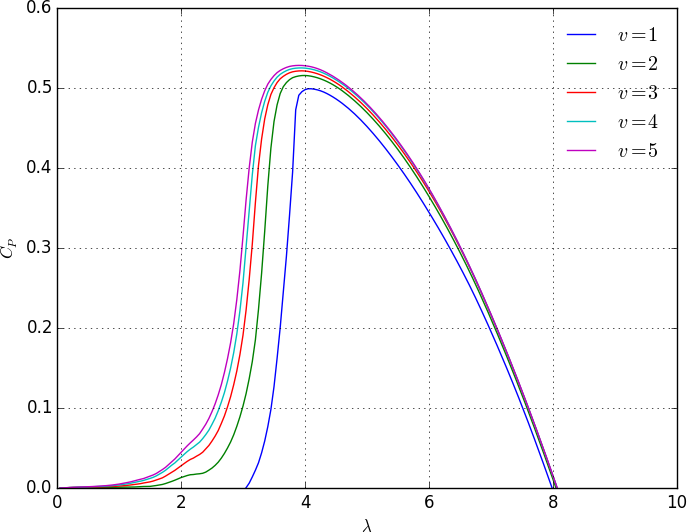
\includegraphics[width=\textwidth]{principles/vawtCp.png}
    \caption{$C_\power(\lambda)$}
    \label{fig:vawtCp}
  \end{subfigure}
  \caption{Estimated performance of a VAWT as a function of wind speed
    $\vel$.}
  \label{fig:vawtSimilarity}
\end{figure}

Consider a vertical axis wind turbine. The most important parameter
for performance is the power $\power = f(R,\rot,\vel,\dens)$, which is
a function
\begin{itemize}
\item the dimensions of the turbine, \eg the radius $R$
\item its rotation speed $\rot$
\item the free stream velocity $\vel$
\item the density of the air $\dens$
\end{itemize}
Figure \ref{fig:vawtSimilarity} shows the power curves for a given
turbine and air density, as a function of rotation speed for several
free stream velocities.

We have 3 dimensions, namely length $L$, time $t$ and mass
$M$. Therefore the Buckingham theorem tells us the performance is
determined by the relation between two non-dimensional parameters. The
choice of these parameters is to some extent arbitrary. Obviously, the
flow around the turbine is mostly determined by the relative speed of
the turbine with respect to the wind, or the \emph{tip speed ratio}:
\begin{align*}
  \lambda = \frac{\rot R}{\vel} \\
\end{align*}
The power coefficient $C_\power$ then indicates the fraction of the
theoretical kinetic energy passing through the frontal surface of the
wind turbine that is converted into power:
\begin{align*}
  C_\power = \frac{\power}{\frac{1}{2} \dens \vel^3 2 R H}
\end{align*}
We will later see that $C_\power$ is subject to the \emph{Betz} limit,
\ie $C_\power \leq 0.59$. In practice, the maximum power is still
further limited due to the fact that at very low rotation speeds, the
wind turbine needs to divert the air flow much more, leading to higher
kinetic energy losses; this determines the \emph{Schmitz} limit.

When plotting the power coefficient versus tip speed ratio $C_\power=
C_\power(\lambda)$, the curves for the different wind speeds almost
perfectly collapse. There are slight differences because we willingly
neglected one effect: the viscosity. If we would have done so, the
performance would be described by the relationship $C_\power =
C_\power(\lambda,Re)$, with $Re$ an appropriately chosen Reynolds
number. However, the curves indicate that the Reynolds-number
dependence is rather weak and only a second order effect.

\begin{figure}[!h]
  \centering
  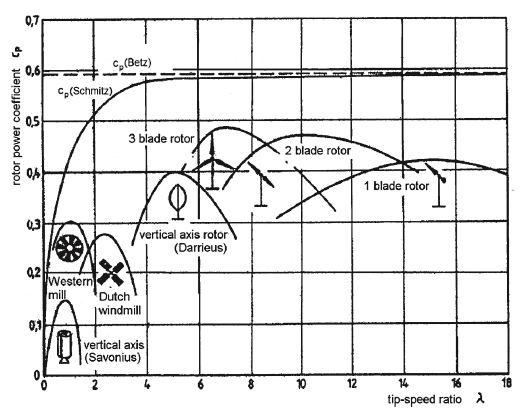
\includegraphics[width=0.7\textwidth]{principles/wt_types_ifo_tsr.png}
  \caption{choice of wind turbine type as a function of tip speed ratio}
  \label{fig:choiceWT}
\end{figure}
Now we can go one step further. We see that the collapsing curves in
figure \ref{fig:vawtCp} all have a common maximum at a given
$\lambda_d \approx 4$, (hopefully) corresponding to the design
point. We can now associate its optimal value and the corresponding
$C_\power$ to characterize the machine geometry. Obviously, this
association is not bijective. $\lambda_d$ is then called the tip speed
ratio of the machine. One should clearly distinguish $\lambda$,
characterising an operation point for a given machine, from
$\lambda_d$ which characterizes geometry.

We can then collect these performance pairs in a single plot, shown in
figure \ref{fig:choiceWT}, and compute the envelope of maximally
obtained $C_\power$ as a function of $\lambda_d$. This plot can then
be used to choose the optimal geometry and tip speed ratio for given
operating conditions.

%%% Local Variables: 
%%% mode: latex
%%% TeX-master: t
%%% End: 
